\section{Methods}\label{sec:methods}
In this chapter, the methods for investigating a bridge design, verifying its structural safety and estimating its cost are introduced. In Section \ref{sec:met_ref} the Blennerhassett Island Bridge, as well as other reference bridges, are presented.
Section \ref{sec:met_str} introduces the structural model and briefly assesses its underlying assumptions. Further, an overview of the investigated load cases is given in Section \ref{sec:met_loads}. The determination of the self-equilibrium stress state is of critical importance. The designer can freely assign it to the structure, contrary to the load cases, whose effects are determined by the elastic response of the structure. Section \ref{sec:met_seq} describes different methods to obtain this state which also includes the choice of the arch shape. The limit states for the design criteria as well as the corresponding verifications are specified in Section \ref{sec:met_ver}, combining the self-equilibrium stress state with the factored load cases. Based on these verifications, the cost of an investigated design is estimated according to Section \ref{sec:met_cost}. The methods presented in this chapter are exemplified by the final design of the Blennerhassett Island Bridge based on the design drawings.

\subsection{Reference bridges} \label{sec:met_ref}

\newpage
\subsection{Structural model} \label{sec:met_str}
A defining feature of the Blennerhassett Island Bridge is the floating deck. It is supported only at the 13 floor beams and acts as almost structurally independent and resembles a bridge on by itself. Compared to a composite deck, it causes a certain inefficiency in material use and the additional arrangement of many bearings. On the other hand, it allows for a replacement of the deck in the future and it simplifies the investigation of the flow of forces. It carries the loads over a span of 20 meters to the adjacent floor beams. There, the forces are mainly carried by the respective hanger pair and partially by the tie girder. This feature allows for a separation of the behaviour of the remaining network arch from the deck. As it is not the objective of this Thesis to investigate and optimise the deck system it is not further considered. The structural model of the network tied-arch bridge is therefore composed of the tie, the arch and the hangers. According to Smit, the behaviour of the two planes of the arch can be considered decoupled from each other \citep{Smit}. Therefore, the behaviour of the arch is analysed in a single arch plane.\medskip

In the design drawings, the structure is divided into segments for the arch and the tie. Each of these segments is verified independently in the design verifications. This segmentation, which is shown along with the bridge in Figs. \ref{fig:Blennerhassett2_a} and \ref{fig:fig:Blennerhassett2_b}, is also used for the analysis in this Thesis.

%On these segments, the maximum degree of compliance, which will determine the cost of each segment, is calculated individually. An overview of the Blennerhassett Island Bridge and its structural model with its segments are shown in Figs. \ref{fig:Blennerhassett2_a} and \ref{fig:fig:Blennerhassett2_b}.

\begin{figure}[H]
\centering
\begin{subfigure}{0.5\textwidth}
    \centering
    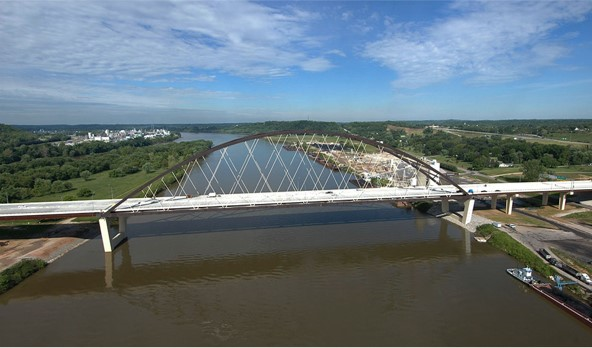
\includegraphics[width=0.9\textwidth]{overleaf/Pictures/Blennerhassett_2.jpg}
    \caption{Built structure}
    \label{fig:Blennerhassett2_a}
\end{subfigure}%
\begin{subfigure}{.5\textwidth}
    \centering
    \vspace*{0.67cm}
    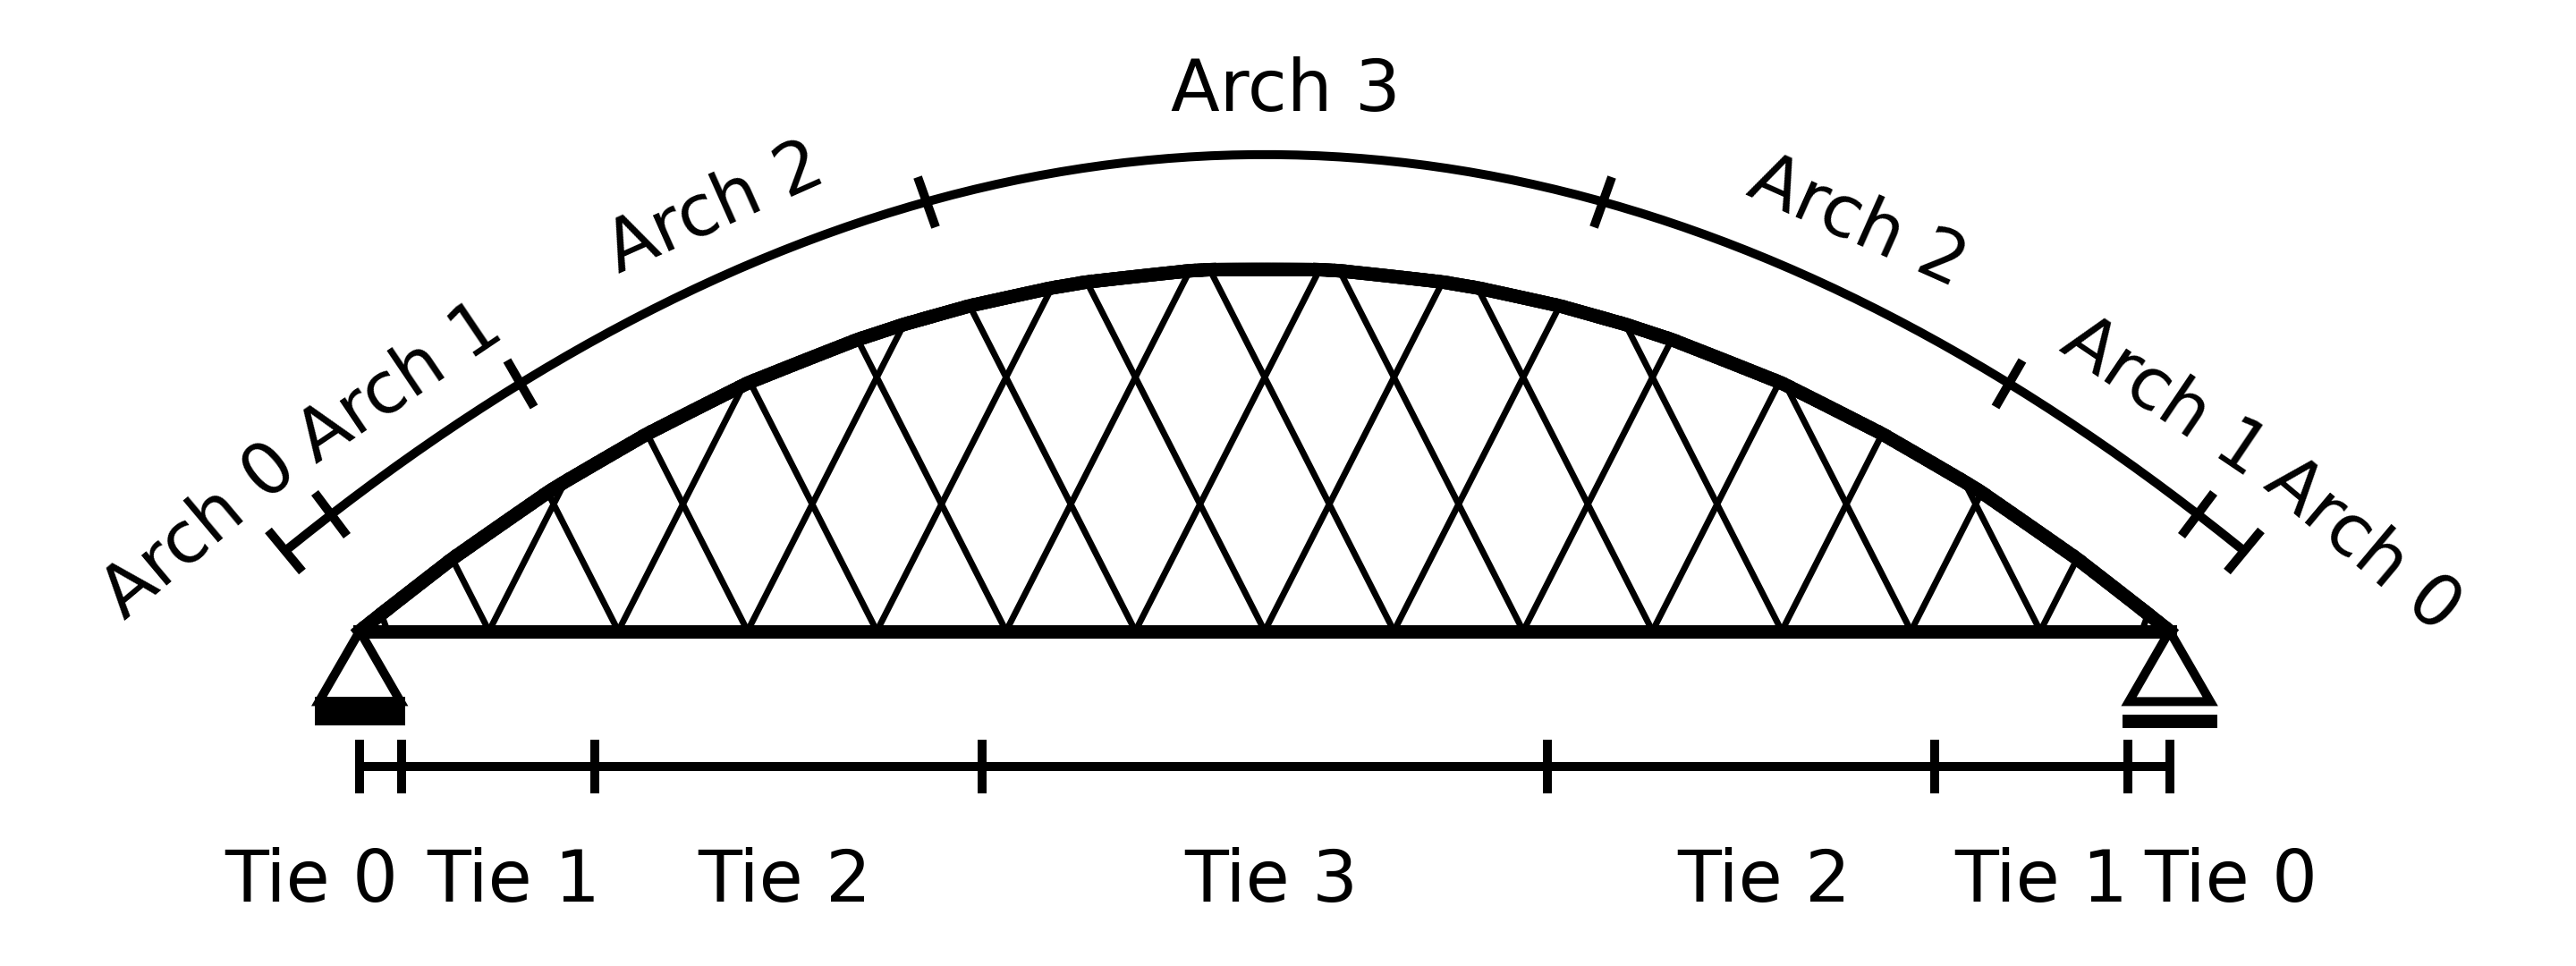
\includegraphics[width=0.9\textwidth]{illustrations/figures/segments.png}
    \vspace*{0.67cm}
    \caption{Structural model and segments}
    \label{fig:fig:Blennerhassett2_b}
\end{subfigure}
\caption{Blennerhassett Island Bridge}
\label{fig:Blennerhassett2}
\end{figure}

The arch and the tie feature different cross-sections in the knuckle region, where the highest internal force effects are expected. The respective stiffnesses are almost twice as high as the stiffness of the field cross-sections.  as presented in Table \ref{tab:cs_stiffnesses}.

Considering their slenderness, the arch and the tie can be accurately modelled as beam elements. On the other hand, secondary effects cannot always be neglected for the hangers because of their low bending stiffness. However, a brief investigation, given in Appendix \ref{Appendix_A_Hangers}, showed that above \SI{100}{MPa} these effects are irrelevant. Therefore, the hangers are modelled as beams with rotational end releases and their self-weight is neglected. Hence, the structure is analysed in the framework of two-dimensional and linear elastic beam statics. The structural analysis is conducted using a python package written by the author of this Thesis in an earlier project.\bigskip


Additionally, there is also a web connecting the tie and the arch at the knuckle, as shown in Figure \ref{fig:knuckle_region}.

\begin{table}[H]
\caption{Cross-sectional stiffnesses}
\label{tab:cs_stiffnesses}
\centering
\begin{tabular}{lccc}
\hline
Segment & Normal stiffness & Bending stiffness & Shear stiffness \\
 & [\SI{}{MN}]   & [\SI{}{MNm^2}] & [\SI{}{MN}] \\ \hline
Arch 1 & \SI{77429}{} & \SI{31473}{} & \SI{79.1}{}\\
Arch 2 & \SI{65997}{} & \SI{28673}{} & \SI{63.4}{}\\
Arch 3-4 & \SI{61814}{} & \SI{28113}{} & \SI{42.7}{}\\
Tie 1 & \SI{77429}{} & \SI{31473}{} & \SI{76.2}{}\\
Tie 2 & \SI{65997}{} & \SI{28673}{} & \SI{56.6}{}\\
Tie 3-4 & \SI{61814}{} & \SI{28113}{} & \SI{45.8}{}\\
Hangers & 643 & - & - \\\hline
\end{tabular}
\end{table}

\begin{figure}[H]
    \centering
    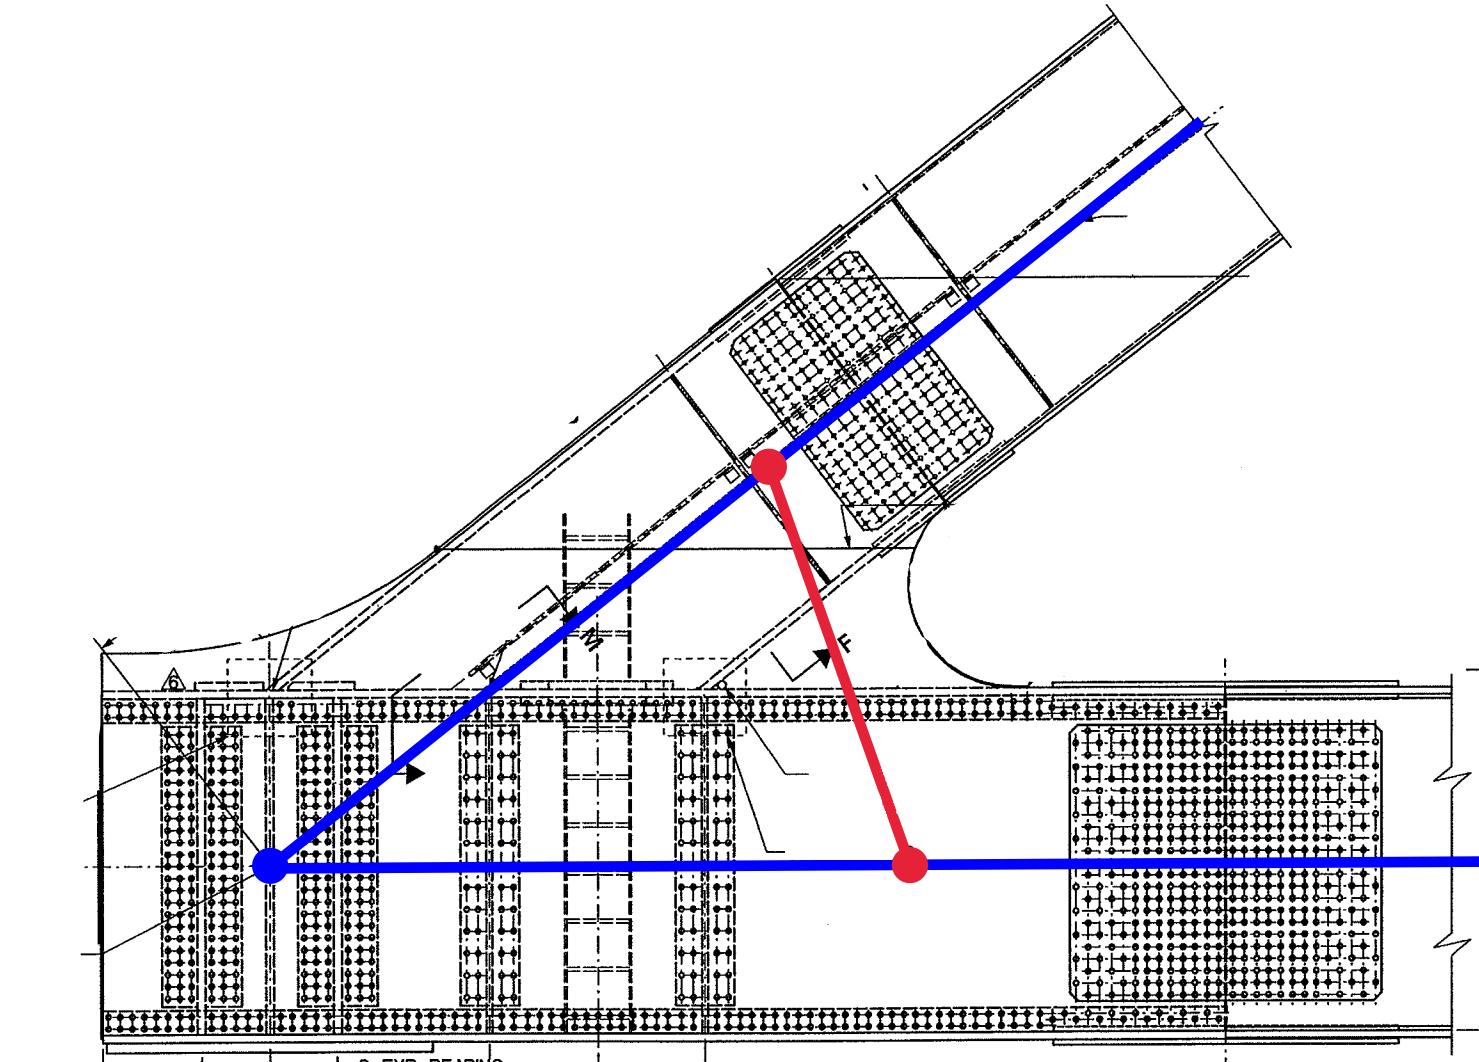
\includegraphics[width=0.8\textwidth]{overleaf/Pictures/Knuckle region.png}
    \caption{Plan and modelling of the knuckle region}
    \label{fig:knuckle_region}
\end{figure}

To judge the influence of these features on the internal force effects, the structure is analysed using different models. In the first model, the field cross-sections are used everywhere and also no web member is considered. In a second model, a web steel member with a cross-section of 0.127m x 1.067m is introduced. Additionally, the actual cross-sections are assigned to the arch and the tie in a third model. The elastic effects under dead loads are compared in Fig. [].
region-wise between the three different models. The results are presented in Table []. [conclusion]

\newpage
\subsection{Load cases} \label{sec:met_loads}
The load cases relevant to this investigation are the dead loading (DL), the live loading (LL) and the wind loading (WS). The dead loading is further subdivided into the weight of the structural components and non-structural attachments (DC) and the weight of the future wearing surfaces and utilities (DW).

\subsubsection{Dead loading}
The dead loads for the Blennerhassett Island Bridge were derived from the estimated bridge quantities of the design drawings. The detailed derivation is given in Appendix [] and the final results are presented in Table \ref{tab:dead_loads}. The weight of the arch and the tie girder are distributed as a constant load along the respective elements. A particularly detailed weight distribution by assigning more weight to the stronger cross-sections near the knuckle is disregarded for. Also the weight of the lateral bracing is distributed along the entire arch for simplicity. The deck weight and its non-structural components make up for the main contribution to the dead loading. The weight of the deck, on the other hand, is applied as a concentrated force at the locations of the cross-girders. The weight of the hangers and its resulting bending moment is relatively small and neglected to facilitate some of the used methods. An illustration of all dead loads applied to the structural model is shown in Fig. \ref{fig:dead_loads}.

\begin{table}[H]
    \centering
    \begin{tabular}{lccccc}
        Component & Arch & Tie & Deck & Utilities & Unit \\ \hline
        Weight & 29.8 & 26.4 & 115.3 & 35.1 & \SI{}{kN/m}
    \end{tabular}
    \caption{Weight per component}
    \label{tab:dead_loads}
\end{table}

\begin{figure}[H]
    \centering
    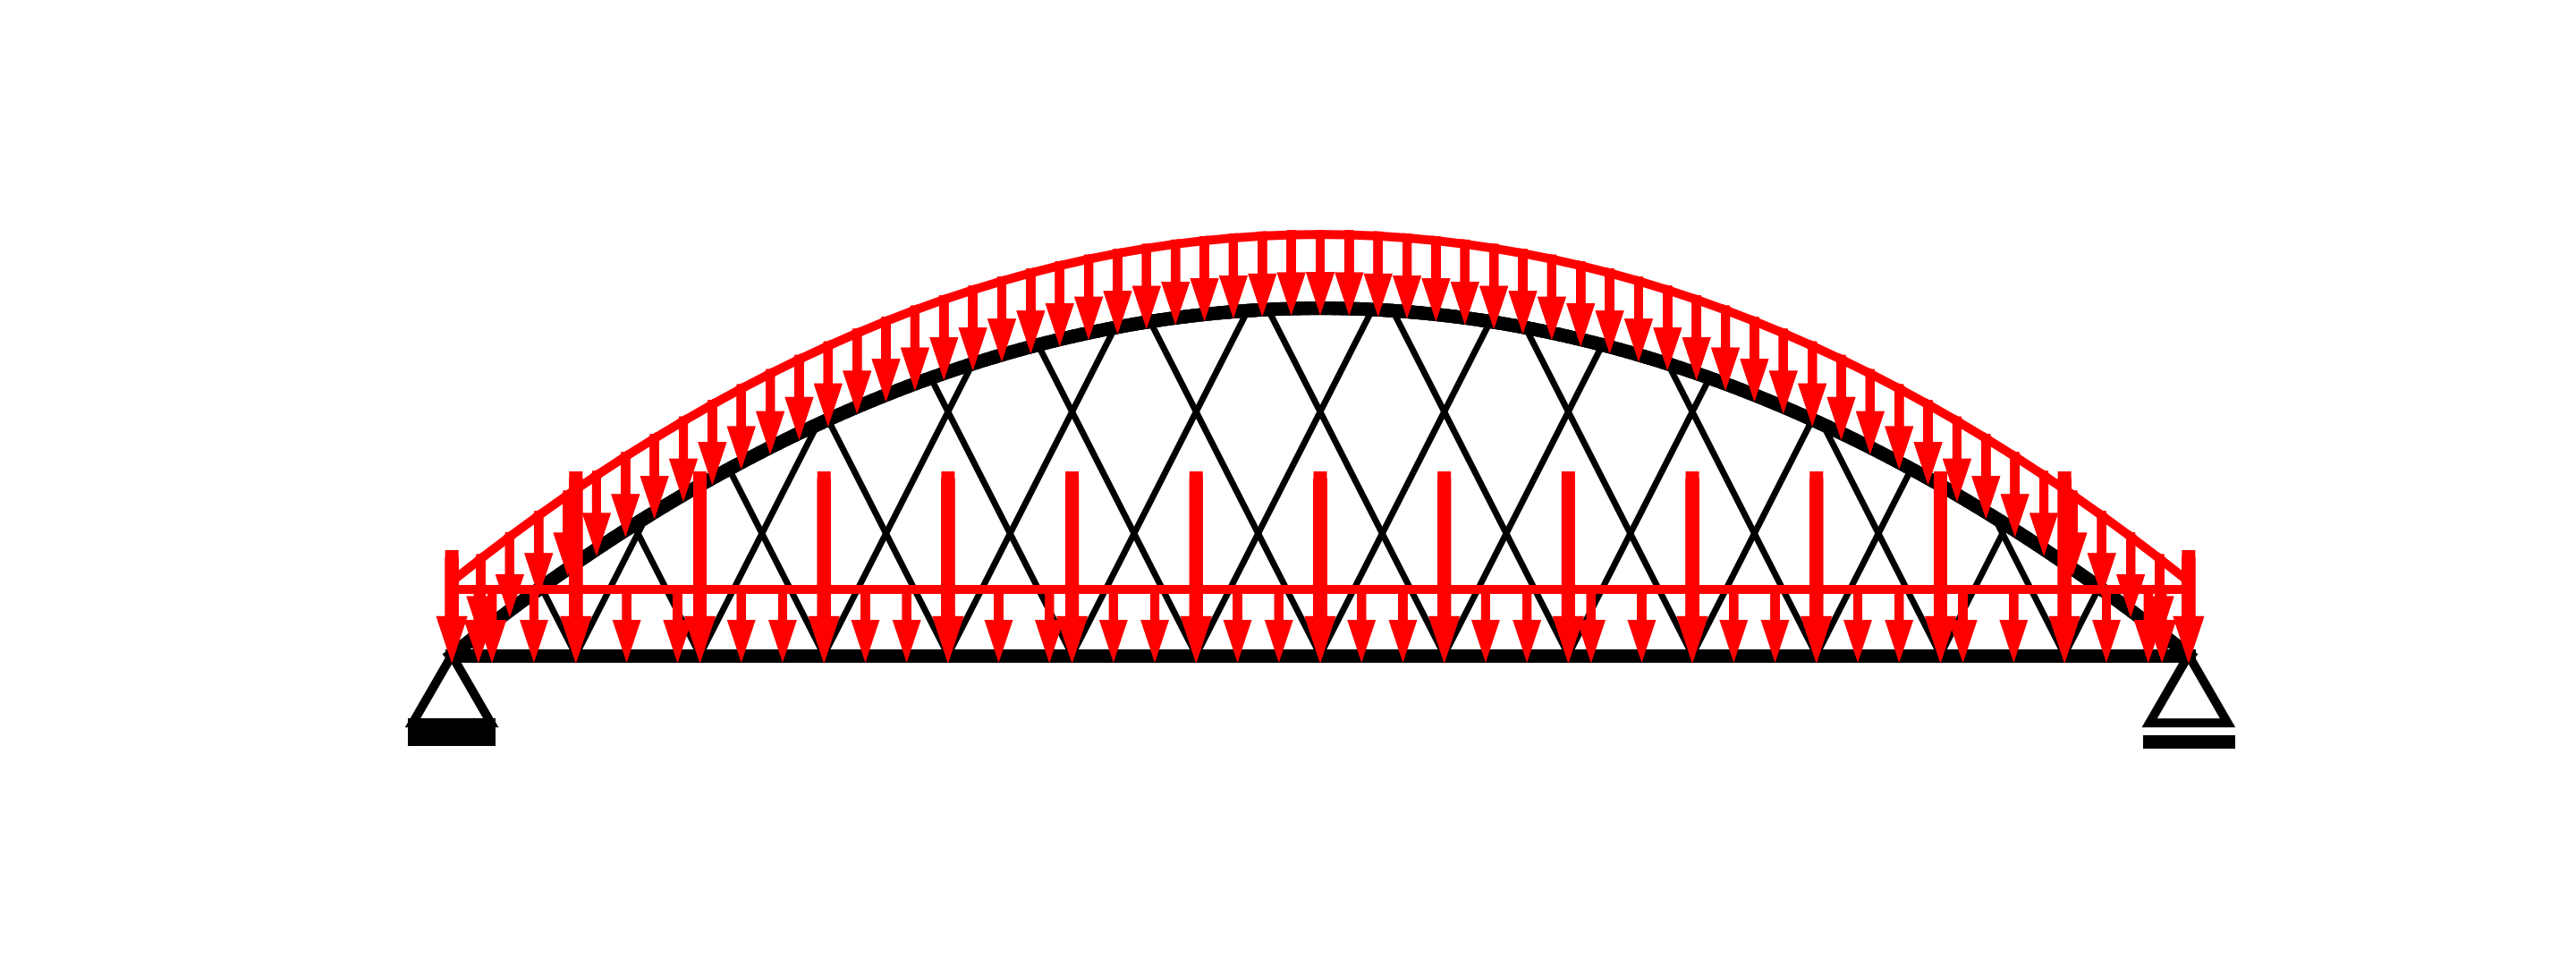
\includegraphics[trim={0 0.8cm 0 0.8cm},clip,
    width=0.8\textwidth]{illustrations/figures/permanent loads.png}
    \caption{Dead loading in the structural model}
    \label{fig:dead_loads}
\end{figure}

\subsubsection{Live loading} \label{sec:met_loads_live}
The load case of live loading is a combination of two separate components. A lane-wise distributed load is applied along the entire or partial length of the bridge and a concentrated truck load is applied at a specific longitudinal point. According to AASHTO code provisions, both loads are factored according to how many lanes they are applied on. Therefore, the number of loaded lanes causing the highest load on one side of the tie girder is determined in a first step. In the detailed calculations in Appendix \ref{Appendix_Liveloading} it can be seen that six loaded lanes cause the largest load in one of the arch planes. This conclusion is also valid for the truck loads which are also applied on six lanes. An overview of the design loads is given in Table \ref{tab:live_load_overview}. 

\begin{table}[H]
\centering
\caption{Overview of the live loading}
\label{tab:live_load_overview}
\begin{tabular}{cccccc}
\begin{tabular}[c]{@{}c@{}}Design\\ lane load\end{tabular} & \begin{tabular}[c]{@{}c@{}}Design\\ truck weight\end{tabular} & \begin{tabular}[c]{@{}c@{}}Lane\\ multiplier\end{tabular} & \begin{tabular}[c]{@{}c@{}}Dynamic\\ multiplier\end{tabular} & \begin{tabular}[c]{@{}c@{}}Distributed\\ design load\end{tabular} & \begin{tabular}[c]{@{}c@{}}Concentrated\\ design load\end{tabular} \\ \hline
\SI{9.3}{kN/m} & \SI{325}{kN} & \SI{2.46}{} & \SI{1.33}{} & \SI{23.0}{kN/m} & \SI{1063}{kN}
\end{tabular}
\end{table}


As the live loads are applied on the deck, they act as concentrated forces on the tie at the location of the cross-girders, as presented in Fig. \ref{fig:Live_load_1} for the fully loaded deck. To find the worst longitudinal arrangement of the live loads, the concentrated forces are applied individually. For each point in the model the partially loaded tie and the concentrated force are then combined to produce maximum effects. The concentrated force is thereby only applied at one cross-girder exclusively, as illustrated in Fig. \ref{fig:Live_load_2}. 

%It yields a range of possible effects for each point on the structural elements. The resulting ranges for the Blennerhassett Island Bridge are presented in Fig. [], where the ranges of the concentrated load and the distributed loads are also shown individually. These results agree well with the effects specified on the design drawings.\bigskip

\begin{figure}[H]
\centering
\begin{subfigure}{0.5\textwidth}
    \centering
    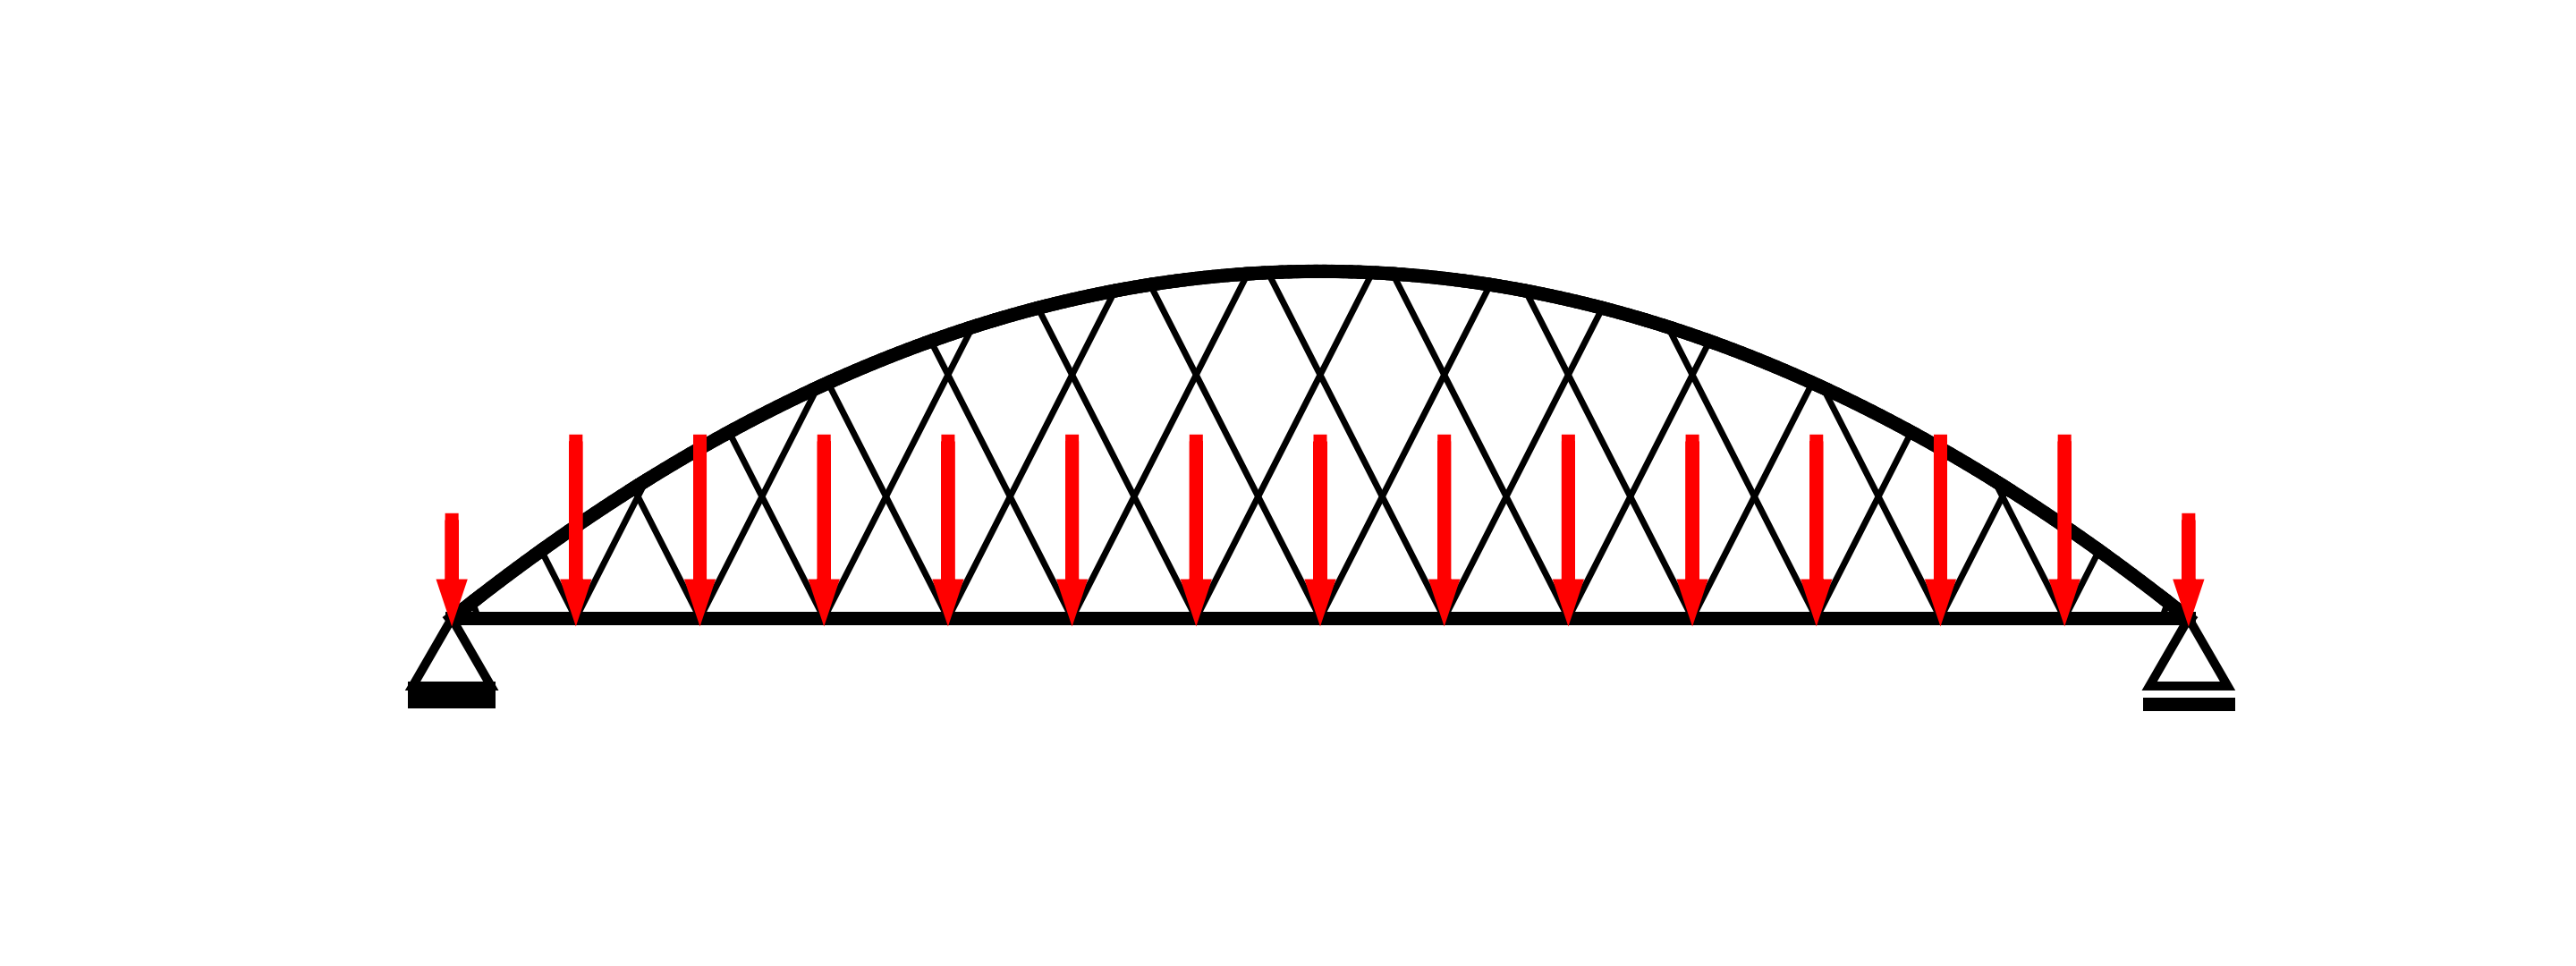
\includegraphics[trim={0 0.8cm 0 0.8cm},clip, width=0.9\textwidth]{illustrations/figures/distributed live loads.png}
    \caption{Distributed live loads}
    \label{fig:Live_load_1}
\end{subfigure}%
\begin{subfigure}{.5\textwidth}
    \centering
    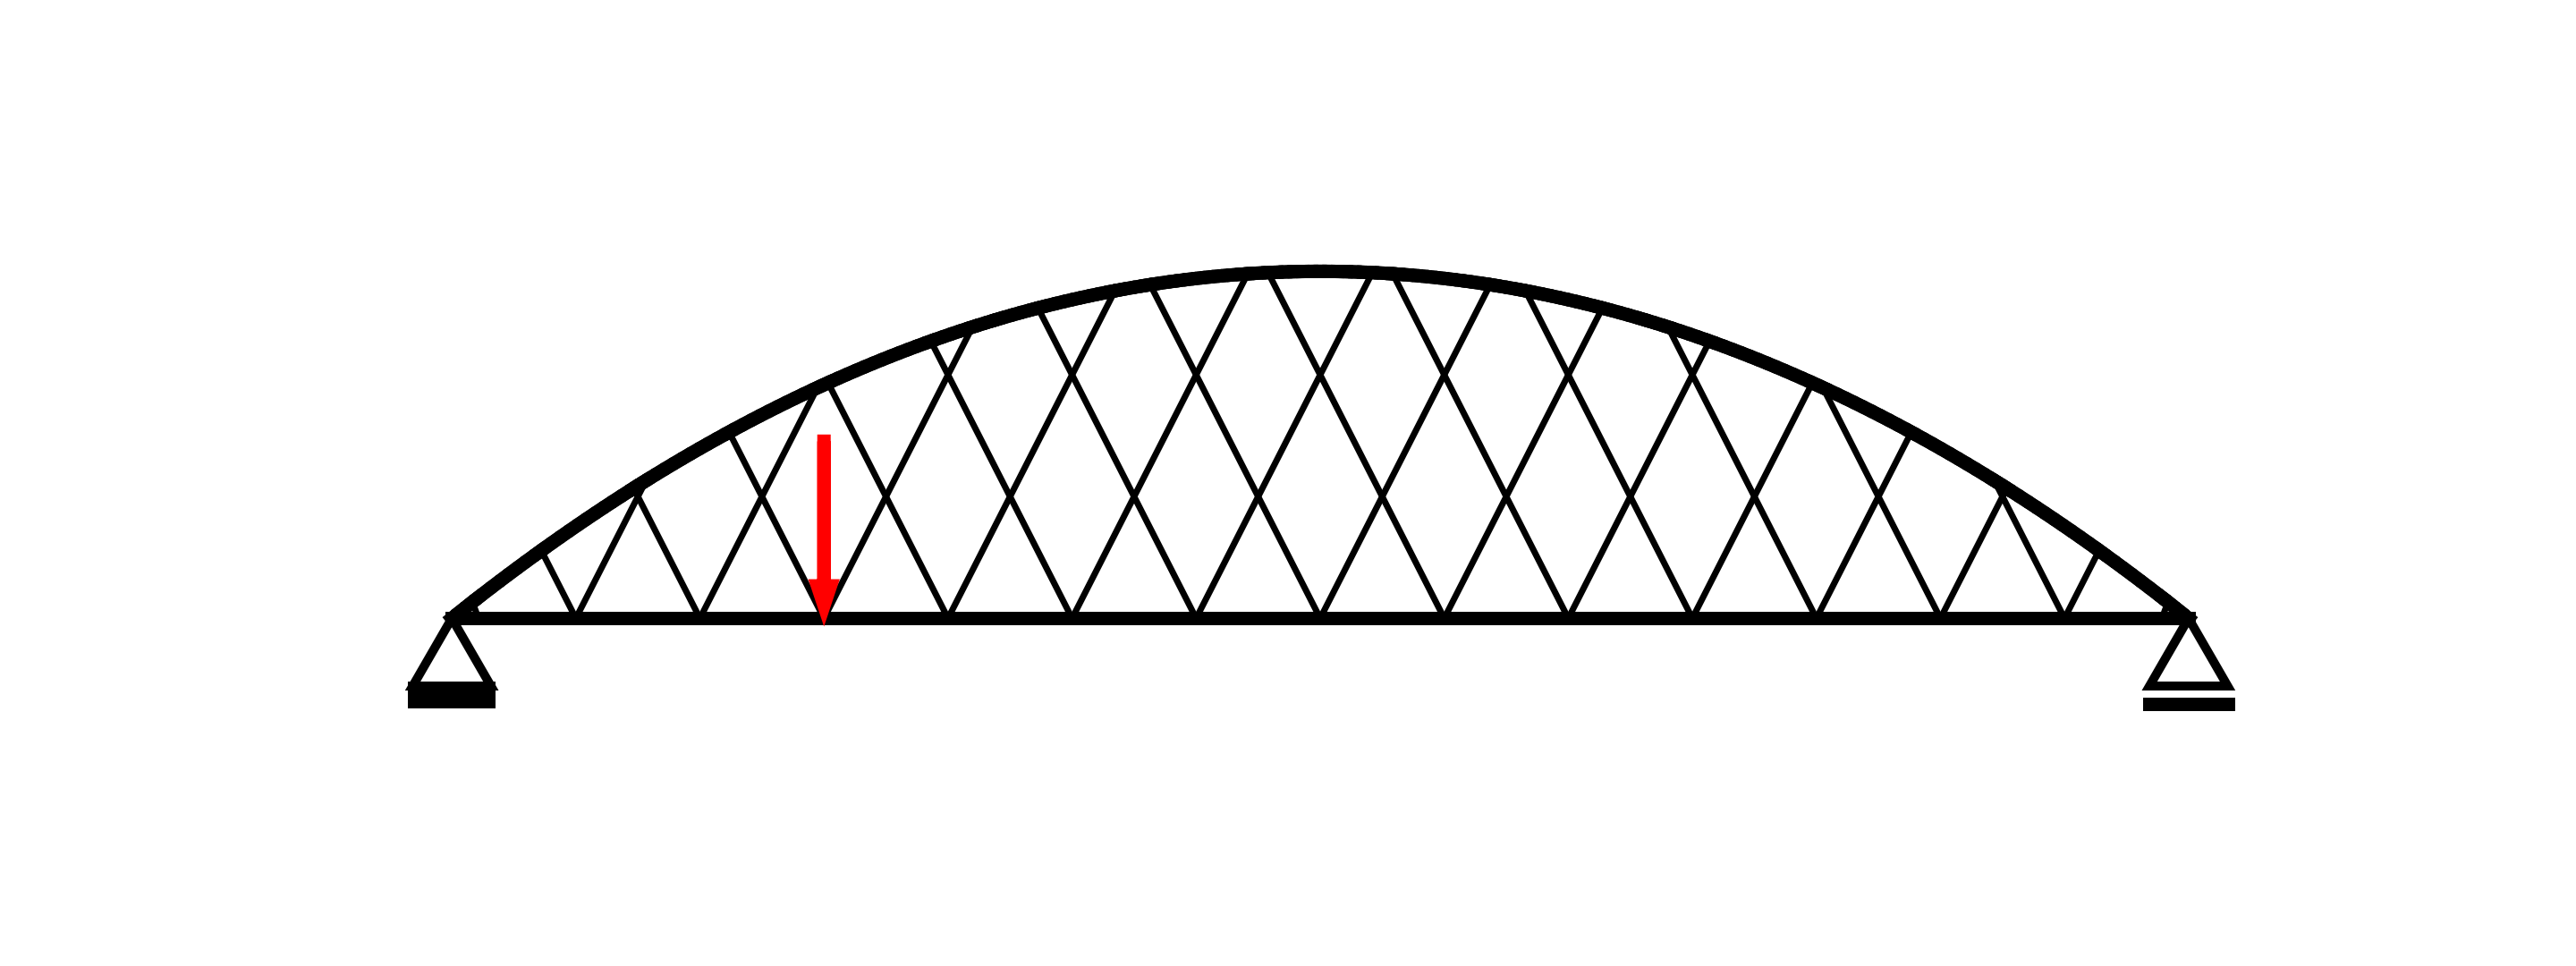
\includegraphics[trim={0 0.8cm 0 0.8cm},clip, width=0.9\textwidth]{illustrations/figures/concentrated live loads.png}
    \caption{Concentrated live loads}
    \label{fig:Live_load_2}
\end{subfigure}
\caption{Live loading in the structural model}
\label{fig:Live_load}
\end{figure}

For the events of cable loss and cable replacement, special circumstances apply to the live loading. For cable loss, it is assumed that only the actually marked lanes are loaded. For cable replacement, one lane is shifted away from the replaced hanger. The determining live load arrangement is calculated and illustrated in the Appendices \ref{Appendx_A_Live_loading_2} and \ref{Appendx_A_Live_loading_3} respectively. The resulting loads on the tie are given in Table \ref{tab:live_load_extreme}. For the event of tie fracture, the same live loading as in the ultimate limit states is applied.

\begin{table}[H]
\centering
\caption{Live loads for extreme events}
\label{tab:live_load_extreme}
\begin{tabular}{lcc}
\hline
Extreme event     & Distributed live load & Concentrated live load \\ \hline
Cable loss  & \SI{14.2}{kN/m} & \SI{660}{kN} \\
Cable replacement & \SI{18.8}{kN/m} & \SI{874}{kN} \\ \hline
\end{tabular}
\end{table}



\subsubsection{Wind loading}
The load case of wind loading is not calculated in this investigation as the loads are particular to a specific design and require a 3-dimensional model. However, the effects specified on the design drawings in the Appendix [] are taken to allow for integral design verifications. The respective characteristic internal force effects under wind loading are shown in Table \ref{tab:effects_wind_load}.

\begin{table}[H] 
\caption{Effects of wind loading per segment}
\label{tab:effects_wind_load}
\centering
\begin{tabular}{lccc}
\hline
Segment & Normal force & Moment-y & Moment-z \\
 & [MN]   & [MNm] & [MNm] \\ \hline
Arch 1 & -7.8 & -0.67 & 10.7\\
Arch 2 & -4.1 & -0.53 & 2.6\\
Arch 3 & -3.9 & 0.12 & 0.11\\
Tie 1 & 7.0 & -1.1 & 5.9\\
Tie 2 & 6.2 & 0.40 & 0.43\\
Tie 3 & 5.3 & 0.70 & 0.79\\
Hangers & 0.48 & - & - \\ \hline
\end{tabular}
\end{table}


%In [] it is mentioned, that the deciding load case for the design of the Blennerhassett Island Bridge is the accidental tie fracture event. It assumes that one of the flanges or the webs of the tie ruptures, which causes immense stresses and strains on the remaining components and also changes the flow of forces. The investigation of this load case lies outside of the scope of this Thesis. Nevertheless, it is indirectly considered in the objective function, which is introduced in Sec. [].

\newpage
\subsection{Self-equilibrium stress state} \label{sec:met_seq}
% Permanent state
In any statically indeterminate structure residual stresses are present when all loads are removed. In the case of a network tied-arch bridge these residual stresses can be controlled by prestressing the hangers and by applying forces to the arch and the tie when the two are closed and locked. The created self-stress state will be present under all following load cases and is in equilibrium with itself. It can be beneficial to counteract the effects expected in the ultimate limit states and is a key factor in the verification of the design conditions. The state can be described by any set of supernumerary forces. For the investigation in this Thesis the supernumerary forces presented in Fig. [] are used. It can be seen that besides the normal forces in the hangers also the moments between the arch and the tie as well as the horizontal force at the right knuckle are part of the set.\\

[Picture]\\

For the Blennerhassett Island Bridge, 29 independent self-equilibrium stress states are present, one for each hanger and three for the arch and the tie. Under consideration of symmetry, 15 independent states remain. Instead of the hypothetical residual stress state under no applied loads, the state under permanent loads is investigated to indirectly define the residual stresses. Whereas for a composite deck under consideration of creeping effects, it makes sense to minimise the permanent bending moments, significant permanent moments can be present in a tie girder with a floating deck. If chosen correctly, they can be facilitating the design verifications. However, the determination of the self-stress state is not straightforward, and many engineers define it by trial and error, as it was the case for the design of the Blennerhassett Island bridge. A few different methods are presented in this Section as well as methods to derive a beneficial arch shape. For the investigation of the stress-state under permanent loads, the structural model of the network arch bridge is split into the tie and the arch. If the forces at the knuckle and in the hangers are consistent, they can ultimately be recombined to form the permanent state of the network arch, as illustrated in Fig. []. \\

[Picture]\\

\subsubsection{Zero-displacement method}
The zero-displacement method is a frequently used first estimation originating from the more popular cable-stayed bridge type. 
The permanent hanger forces are determined from a structural analysis of the girder where at every hanger connection a vertical support is introduced. In this way, the moment distribution in the tie is adequately balanced and creeping effects do not change the moment distribution. For a network tied-arch bridge, additionally to the supports at the connection nodes, a fully fixed support is introduced at the knuckle. It represents the supports of the network arch and also yields a suitable permanent constraint moment at the knuckle. The model of the tie resembles a continuous beam, as shown in Fig. []. For the case of a network tied-arch bridge, multiple hangers can connect to the tie at a particular node and the vertical forces have to be distributed between the two hangers. One option is to assign forces of equal magnitude to each of the hangers resulting in the intended vertical force. 
%As a second option, the hanger forces are assigned proportionally to the hanger length, aiming to achieve similar forces under the ultimate displacement of the tie node.

In a second step, the hanger forces and the constraint moment at the knuckle are applied to the arch to determine its permanent state. Additionally, the permanent tie tension force is applied to it. It can be chosen freely as it was neglected in the investigation of the tie, since it does not affect its moment distribution. For the arch on the other hand, it plays a crucial role. The permanent tie tension force can be calculated to cause a disappearing moment at the crown of the arch according to Eq. []. This approach is illustrated in Fig. []. A second approach, which yields the least-squares solution of the moment distribution in the arch is explained in the Appendix [].

%A simple method to determine thin a way to yield an efficient moment distribution in the arch. For example, it is possible to make the moment at the top of the arch disappear or to obtain a specific moment there. The method is illustrated in Figs [] and []. 


\subsubsection{Moment minimisation}
The moment distribution resulting in the arch according to the previous methods is very unfavourable. Even by optimising the tension force in the tie, the extrema of the moment distribution on the arch are severe. There are two approaches to overcome this issue. An elegant way of reducing the bending moments in the arch is to adapt its shape to the thrust line under permanent loads. This approach is presented in Sec. []. If the shape of the arch is not subject to the optimisation, the only option to improve the moment distribution is by adapting the hanger forces. It is a very challenging task and is usually tackled by the engineer through trial and error. For example, this was the case for the Blennerhassett Island Bridge. Therefore it is challenging to reproduce its prestressing forces for the final design. A similar result is obtained by solving an optimisation problem aiming to minimise the absolute moment maximum in the arch and the tie. This problem is efficiently solvable as it can be formulated as a linear programming problem. The initial guess is obtained by the zero displacement method, and the bounds for the hanger forces are set within a specific range.  The thereby obtained hanger forces and moment distribution resembles the ones the Blennerhassett Island Bridge reasonably well, as shown in Table [].

\subsection{Arch shape} \label{sec:met_arch}

\newpage
\subsection{Design verifications} \label{sec:met_ver}
To ensure a safe and reliable structure, the limit states for strength, extreme events and fatigue are considered \citep{AASHTO}.  The resulting demand over capacity ratios (D/C) will also be used in Section \ref{sec:met_cost} for an estimation of the cost function.

\subsubsection{Strength limit states}
The strength limit states are considered to ensure that the design of the structure guarantees enough strength and stability for the highest expected loads in its life cycle. The load combinations considered in this investigation are related to the main actions of vehicular use (Strength-I), wind exposure (Strength-III) and a load combination for heavy bridges (Strength-IV). The load factors used for each strength limit state are presented in Table \ref{tab:uls_combination}. For the permanent loads DC and DW, two factors are given out of which the one impeding to the verification is taken. For the locked-in erection stresses no variability is taken into account.

\begin{table}[H]
\caption{Load combinations for the ultimate limit state}
\centering
\begin{tabular}{lccccc}
\hline
Load         & EL  & DC         & DW         & LL   & WS  \\ \hline
Strength-I   & 1.0 & 0.9 / 1.25 & 0.65 / 1.5 & 1.75 & -   \\
Strength-III & 1.0 & 0.9 / 1.25 & 0.65 / 1.5 & -    & 1.4 \\ 
Strength-IV  & 1.0 & 0.65 / 1.5 & 0.65 / 1.5 & -    & - \\ \hline
\end{tabular}
\end{table}

The arch and the tie are verified according to Eq. \eqref{eq:design_verification}, neglecting the secondary force effects. For the hangers, enough resistance is proved if the highest stresses are below 65\% of the nominal capacity. 

\begin{equation}
    \frac{N_{Ed}}{N_{Rd}} + \frac{8.0}{9.0}\, \left(\frac{M_{y,Ed}}{M_{y,Rd}}+\frac{M_{z,Ed}}{M_{z,Rd}} \right) \leq 1.0
    \label{eq:design_verification}
\end{equation}

For simplicity, the value given by the left side of this condition is also referred to as the demand over capacity ratio for the arch and the tie.
%For the Blennerhassett Island Bridge, the DOC is evaluated according to this simplified verification. The obtained values are presented in Table [], along with the ratios taken from the design drawings in parenthesis. 

\subsubsection{Extreme event limit states}
Extreme events are unique circumstances whose return periods can be significantly greater than the life expectancy of the structure. In these events, the requirement for the bridge is its structural survival. In this investigation the extreme events of cable loss, cable replacement and tie fracture are examined. The load factors for each event is taken from the design drawings and presented in Table \ref{tab:extreme_combination}. For the events of cable loss and cable replacement, specific live loading arrangements (LL*) apply.

\begin{table}[H]
\caption{Load combinations for the extreme event limit states}
\label{tab:extreme_combination}
\centering
\begin{tabular}{lccccc}
\hline
Event         & EL  & DC         & DW         & LL*   & DAF  \\ \hline
Cable loss   & 1.0 & 1.2 & 1.4 & 0.75 & 1.75   \\
Cable replacement & 1.0 & 1.2 & 1.4 & 1.5 & 1.0 \\ 
Tie fracture  & 1.0 & 1.25 & 1.5 & 1.3 & - \\ \hline
\end{tabular}
\end{table}

For both hanger-related extreme events, each hanger is investigated individually according to the PTI (static) approach [cite PTI]. In a first step, the longitudinal live load arrangement, which maximises the respective hanger force, is determined. Therefor, The concentrated live load is always applied at the cross-girder closest to the considered hanger. The forces from the distributed live load are also arranged on a certain amount of neighbouring cross-girders, as illustrated in Fig. \ref{fig:Cable_Loss_1}. The assumed hanger force before its replacement or loss is thereby determined. In a second step, the structural system is modified by removing the considered hanger. The hanger force is applied in opposite direction on the modified system, as shown in Fig. \ref{fig:Cable_Loss_2}. The resulting effects are multiplied by a dynamic amplification factor (DAF) and superimposed on the effects from the state of maximised hanger force. The DAF for the event of cable loss is assumed to be 1.75.\\

\begin{figure}[H]
\centering
\begin{subfigure}{0.5\textwidth}
    \centering
    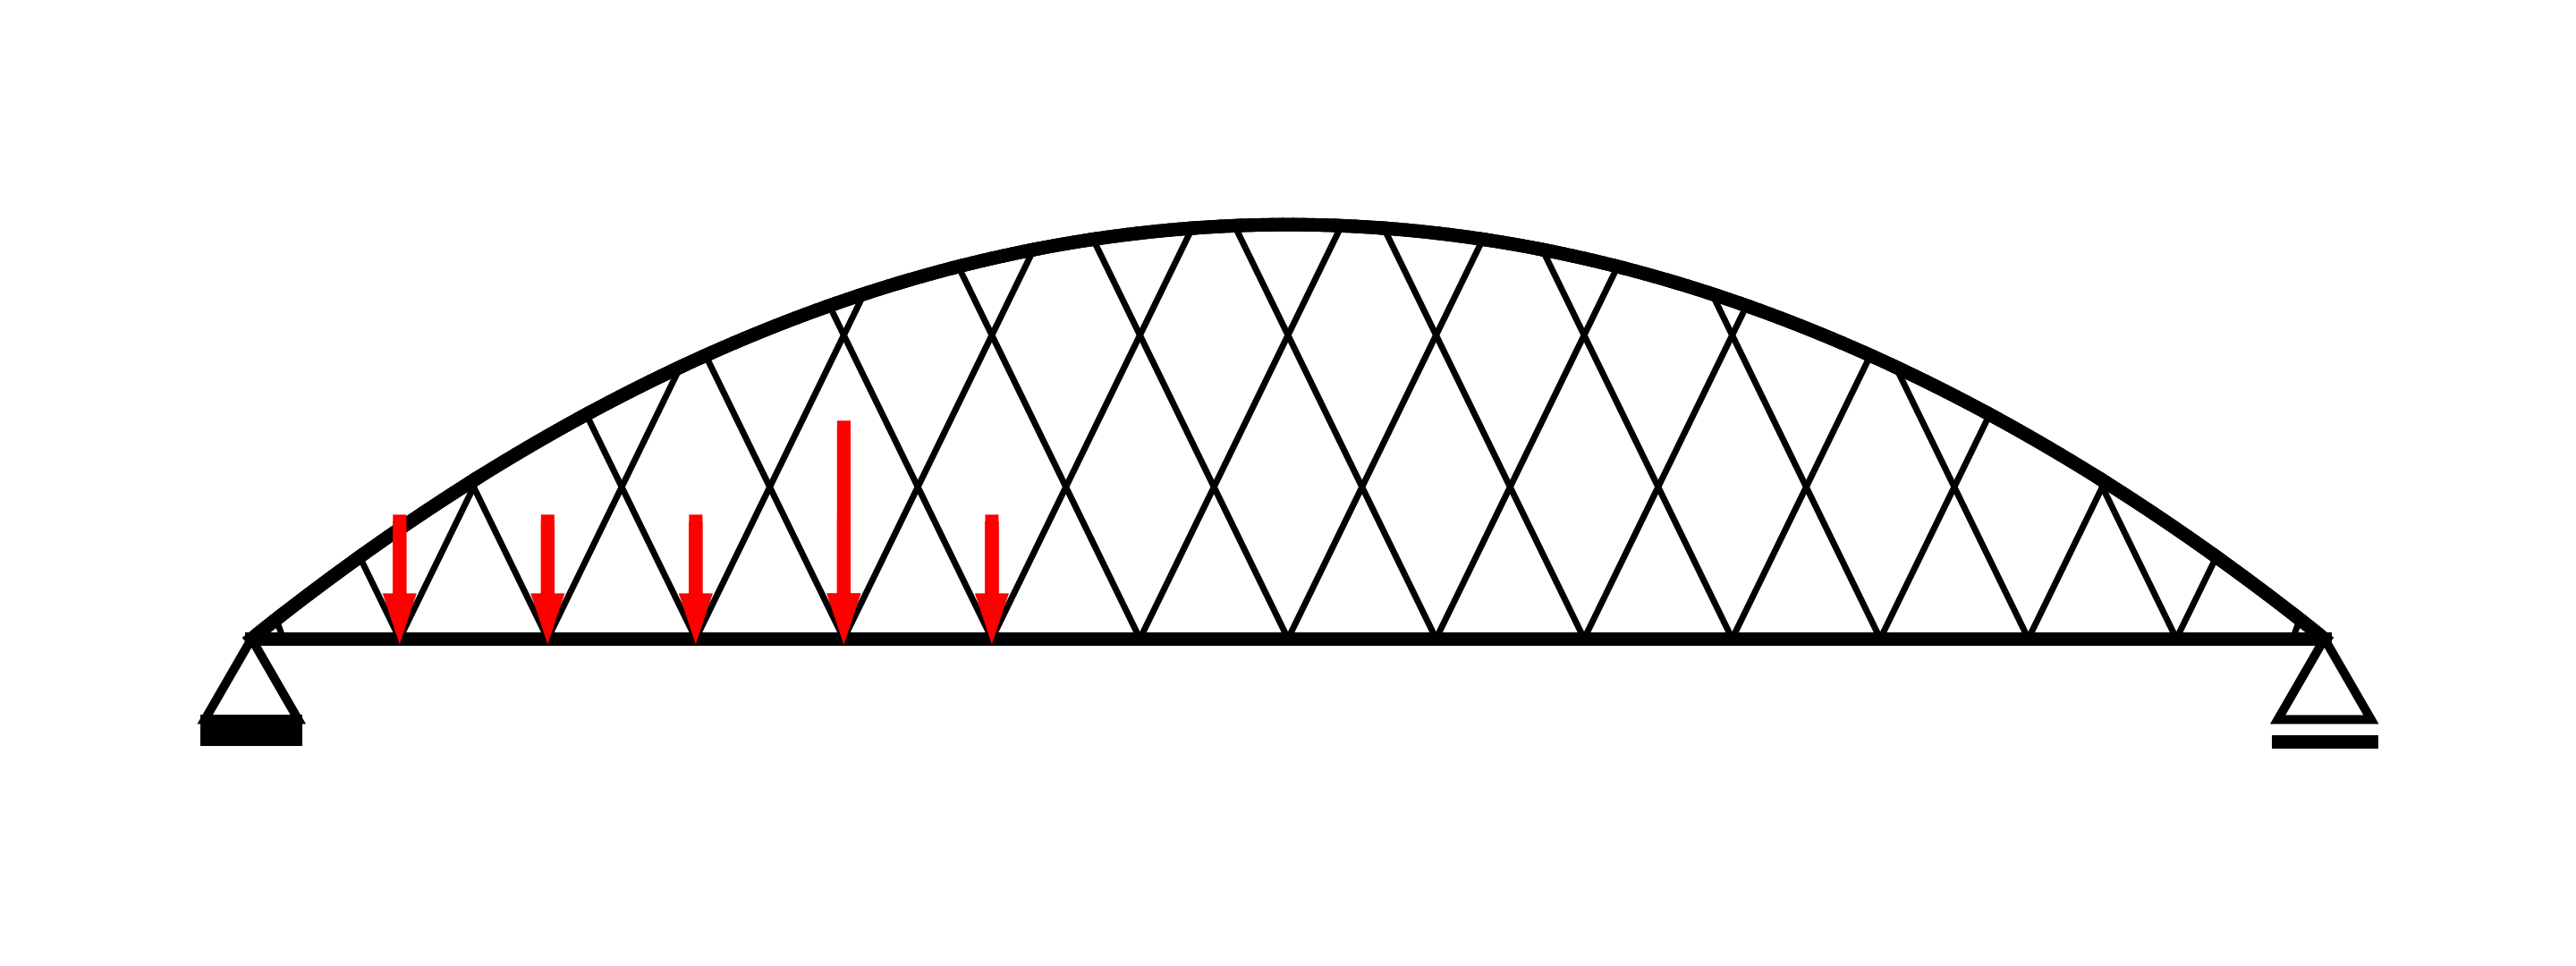
\includegraphics[trim={0 0.8cm 0 0.8cm},clip, width=0.9\textwidth]{illustrations/figures/cable loss - load arrangement.png}
    \caption{Live load arrangement to maximise hanger force}
    \label{fig:Cable_Loss_1}
\end{subfigure}%
\begin{subfigure}{.5\textwidth}
    \centering
    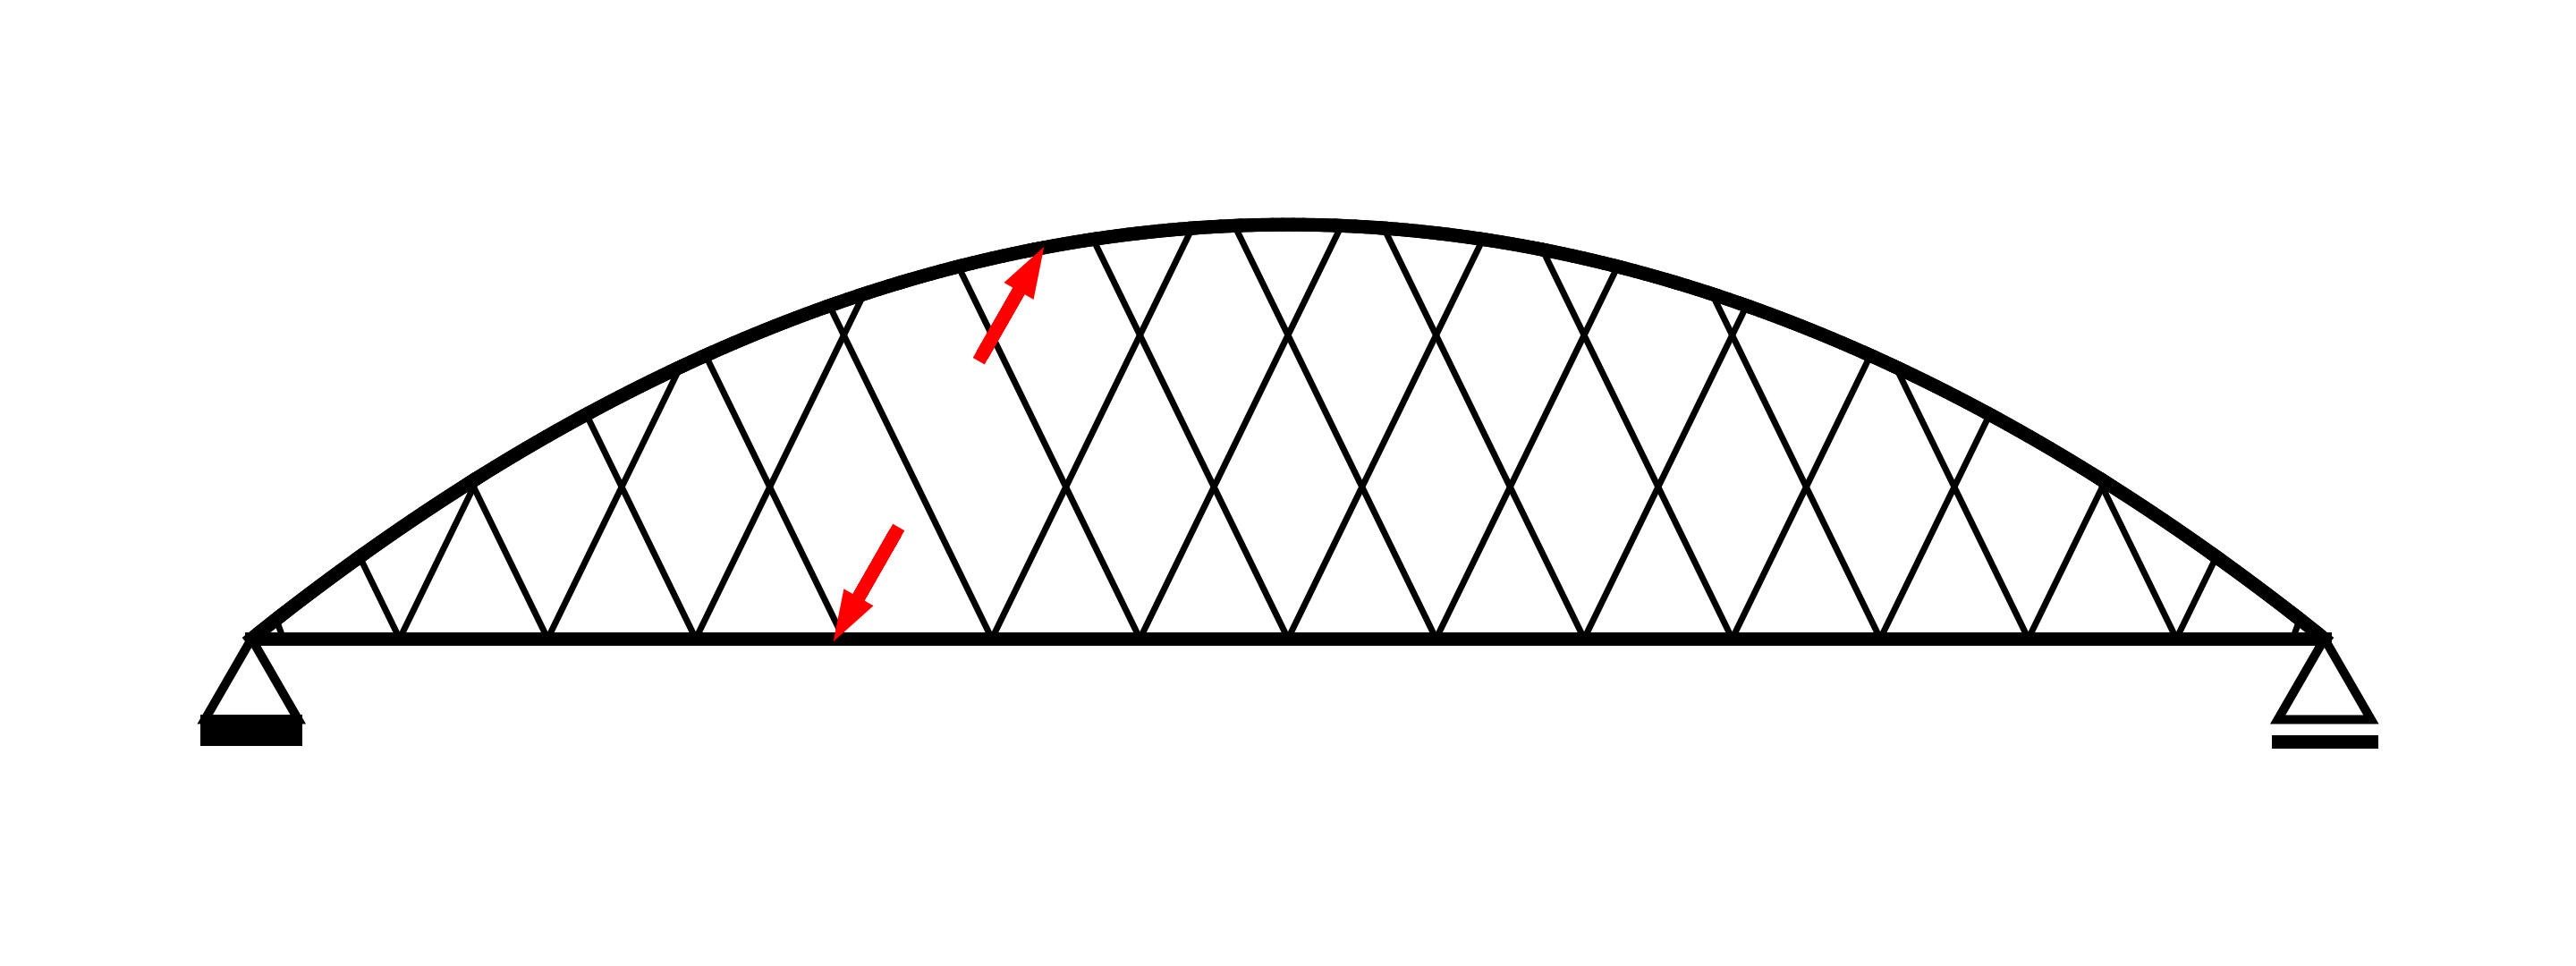
\includegraphics[trim={0 0.8cm 0 0.8cm},clip, width=0.9\textwidth]{illustrations/figures/cable loss.png}
    \caption{Structural model with opposite force}
    \label{fig:Cable_Loss_2}
\end{subfigure}
\caption{Calculation steps for loss of the fourth hanger}
\label{fig:Cable_Loss}
\end{figure}

[Tie fracture]

\subsubsection{Fatigue limit state}

\begin{table}[H] 
\caption{Cross-sectional resistances}
\centering
\begin{tabular}{lccc}
\hline
Segment & Normal force & Moment-y & Moment-z \\
 & [MN]   & [MNm] & [MNm] \\ \hline
Arch 1 & \SI{130.0}{} & \SI{78.7}{} & \SI{79.1}{}\\
Arch 2 & \SI{108.8}{} & \SI{71.5}{} & \SI{63.4}{}\\
Arch 3-4 & \SI{82.3}{} & \SI{50.0}{} & \SI{42.7}{}\\
Tie 1 & \SI{153.2}{} & \SI{100.8}{} & \SI{76.2}{}\\
Tie 2 & \SI{117.1}{} & \SI{82.8}{} & \SI{56.6}{}\\
Tie 3-4 & \SI{100.6}{} & \SI{76.2}{} & \SI{45.8}{}\\
Hangers & 4.19 & - & - \\\hline
\end{tabular}
\end{table}

\subsection{Estimation of cost function} \label{sec:met_cost}
